%! Author = Omar Iskandarani
%! Title = Einstein and the Æther: A Philosophical Foundation for the Vortex Æther Model (VAM)
%! Date = May 23, 2025
%! Affiliation = Independent Researcher, Groningen, The Netherlands
%! License = © 2025 Omar Iskandarani. All rights reserved. This manuscript is made available for academic reading and citation only. No republication, redistribution, or derivative works are permitted without explicit written permission from the author. Contact: info@omariskandarani.com
%! ORCID = 0009-0006-1686-3961
%! DOI = 10.5281/zenodo.15566101
%! Author = Omar Iskandarani
%! Date = 2025-06-13

% === Metadata ===
\newcommand{\papertitle}{Defining Temporal Constructs in the Vortex Æther Model (VAM)}
\newcommand{\paperauthor}{Omar Iskandarani}
\newcommand{\paperaffil}{Independent Researcher, Groningen, The Netherlands}
\newcommand{\paperdoi}{10.5281/zenodo.15566319}
\newcommand{\paperorcid}{0009-0006-1686-3961}

\ifdefined\standalonechapter\else
  % Standalone mode
  \documentclass[12pt]{article}
  \usepackage[a4paper, margin=2cm]{geometry}
  \usepackage{ifthen} % we can use it safely now
  \usepackage{import}
  \usepackage{subfiles}
  \usepackage{hyperref}
  \usepackage{graphicx}
  \usepackage{amsmath, amssymb, physics}
  \usepackage{siunitx}
  \usepackage{tikz}
  \usepackage{booktabs}
  \usepackage{caption}
  \usepackage{array, tabularx}
  \usepackage{listings}
  \usepackage{bookmark}
  \usepackage{newtxtext,newtxmath}
  \usepackage[scaled=0.95]{inconsolata}
  \usepackage{mathrsfs}
  % vamappendixsetup.sty

\newcommand{\titlepageOpen}{
  \begin{titlepage}
  \thispagestyle{empty}
  \centering
  {\Huge\bfseries \papertitle \par}
  \vspace{1cm}
  {\Large\itshape\textbf{Omar Iskandarani}\textsuperscript{\textbf{*}} \par}
  \vspace{0.5cm}
  {\large \today \par}
  \vspace{0.5cm}
}

% here comes abstract
\newcommand{\titlepageClose}{
  \vfill
  \null
  \begin{picture}(0,0)
  % Adjust position: (x,y) = (left, bottom)
  \put(-200,-40){  % Shift 75pt left, 40pt down
    \begin{minipage}[b]{0.7\textwidth}
    \footnotesize % One step bigger than \tiny
    \renewcommand{\arraystretch}{1.0}
    \noindent\rule{\textwidth}{0.4pt} \\[0.5em]  % ← horizontal line
    \textsuperscript{\textbf{*}}Independent Researcher, Groningen, The Netherlands \\
    Email: \texttt{info@omariskandarani.com} \\
    ORCID: \texttt{\href{https://orcid.org/0009-0006-1686-3961}{0009-0006-1686-3961}} \\
    DOI: \href{https://doi.org/\paperdoi}{\paperdoi} \\
    License: CC-BY 4.0 International \\
    \end{minipage}
  }
  \end{picture}
  \end{titlepage}
}
  \begin{document}

  % === Title page ===
  \titlepageOpen

  \begin{abstract}

This appendix derives and interprets key temporal field equations within the Vortex Æther Model (VAM), a framework that integrates fluid dynamics, topology, and field theory to describe spacetime as a rotating superfluid medium. By introducing constructs such as Swirl Clock phase, Aithēr-Time, and Vortex Proper Time, we explore the dynamical interplay between internal vortex evolution and external ætheric modulation. The appendix provides derivations for three cornerstone equations: energy conservation with Kairos-event triggering, phase-gradient dynamics of the swirl clock, and field tensor modulation in an æther-relative frame. Each expression is linked to a physically motivated symmetry or conservation principle, offering insight into how temporality and topological coherence co-emerge in this model. These results pave the way for quantized time constructs and vortex-based interpretations of mass, gravity, and field interaction.

  \end{abstract}

  \titlepageClose
\fi

% ============= Begin of content ============
\section{\papertitle}

In the Vortex Æther Model (VAM), time is not singular—it is layered, emergent, and topologically mediated. To account for the various temporal phenomena observed in knotted fluid structures and relativistic motion, we introduce a multi-tiered temporal ontology.

  \begin{figure}[h]
    \centering
    \includegraphics[width=0.75\textwidth]{../images/TimeConstruct}
    \caption{Ontological spiral of temporal emergence in the Vortex Æther Model, illustrating the transition from absolute ætheric time to vortex-local and emergent moments.}
    \label{fig:temporal_swirl}
\end{figure}


\noindent As shown in Figure~\ref{fig:temporal_swirl}, each form of time flows outward from the center—the \textbf{Æther Origin}—along an ontological spiral:
$$ \mathcal{N} \longrightarrow \nu_0 \longrightarrow \tau \longrightarrow S(t) \longrightarrow T_v \longrightarrow \mathbb{K} $$
\begin{enumerate}
    \item \textbf{Æther Frame \( \Xi_0 \)}:   Hypothetical inertial frame where the æther medium is at rest. Used for symmetry-breaking and baseline flow analysis.
    \item \textbf{Aithēr-Time\( \mathcal{N} \)}: The foundational, universal time. It is absolute, metaphysical, and unmeasurable. All other forms of time emerge in relation to it.
    \item \textbf{Now-Point \( \nu_0 \)}: The intersection of a local system with the universal present. It serves as a temporal 'event horizon'—a delta-function sampling of \( \mathcal{N} \).

    \item \textbf{Chronos-Time \( \tau \)}: Measurable, proper time experienced by observers moving through the æther. Subject to dilation effects; it arises from a sequence of Now-Points.

    \item \textbf{Swirl Clock \( S(t) \)}: The cyclical phase of a vortex structure. This internal clock governs identity preservation and rotation-state in the knot.

    \item \textbf{Vortex Proper Time \( T_v \)}: Time internal to a knotted loop, arising from its geodesic closure. Reflects the memory of internal twist and topological persistence.

    \item \textbf{Kairos Moment \( \mathbb{K} \)}: A critical, emergent moment—often tied to topological transitions, bifurcations, or irreversible events such as vortex reconnection.
\end{enumerate}

Together, these constructs model time not as a single axis, but as a woven gradient—from cosmic invariance to local transformation. This spiral encapsulates both the metaphysical foundations and the measurable dynamics of time within the VAM framework.




    \begin{table}[h]
        \centering
        \begin{tabular}{|l|c|l|p{7cm}|}
            \hline
            \textbf{Name} & \textbf{Symbol} & \textbf{Type} & \textbf{Description and Role} \\
            \hline
            Chronos-time & $\tau$ & Relative / Measurable & Sequential time; proper time experienced by localized systems in motion through the æther. Core for modeling time dilation. \\
            \hline
            Aithēr-time & $\mathcal{N}$ & Absolute / Universal & The invariant universal present; a metaphysical and ontological background for all temporal flow. \\
            \hline
            Swirl Clock & $\circlearrowleft$ or $S(t)$ & Local / Cyclical & Internal clock-like rhythm of a vortex knot. Tracks phase, rotation, or identity shift through time. \\
            \hline
            Kairos Moment & $\mathbb{K}$ & Threshold / Emergent & The qualitative, transformational moment when a system undergoes critical phase alignment or collapse. \\
            \hline
            Æther Frame & $\Xi_0$ & Reference Frame & Hypothetical inertial frame where the æther medium is at rest. Used for symmetry-breaking and baseline flow analysis. \\
            \hline
            Vortex Proper Time & $T_v$ & Derived / Topological & Time internal to the closed knot or vortex loop. Emerges from geodesic paths and twist topology. \\
            \hline
            Now-Point & $\nu_0$ & Local Event / Temporal Slice & Precise location in spacetime where a point in the æther intersects the universal present. Useful in field causality. \\
            \hline
        \end{tabular}
        \caption{Temporal constructs used in the Vortex Æther Model. These notations distinguish between measurable time, absolute background time, internal vortex phase, and field-causality moments.}
        \label{tab:VAM_time}
    \end{table}

    \begin{align}
        \text{(1) Vortex Proper Time Evolution:}\\
        \quad & \dv{\tau}{\mathcal{N}} = \gamma^{-1}(\vec{v}) \\
        \text{(2) Swirl Clock Gradient:}\\ \quad & \nabla S(t) = \frac{\partial \vec{S}}{\partial \mathcal{N}} + \omega(\tau) \hat{n} \\
        \text{(3) Field Tensor Modulation (Æther-relative):} \\\quad & F^{\mu\nu}(\Xi_0) = \partial^\mu A^\nu - \partial^\nu A^\mu + \phi(\circlearrowleft) \delta^{\mu\nu} \\
        \text{(4) Ætheric Causality Surface:}\\ \quad & \Sigma_{\nu_0} = \{ x^\mu \ | \ \tau(x) = \mathcal{N} \} \\
        \text{(5) VAM Energy Conservation in Æther Frame:}\\ \quad & \dv{E}{\mathcal{N}} + \nabla \cdot \vec{J} = \mathbb{K}(\vec{x}, \tau)
    \end{align}


\section*{🔀 Classical Greek Candidates}
\subsection*{✅ χρόνος (Chronos) — \textit{Linear time}}
\begin{itemize}
\item Sequential, measurable
\item Already used in physics-adjacent language
\item Good for Swirl Clocks
\end{itemize}

\subsection*{✅ καιρός (Kairos) — \textit{Qualitative, sacred, the right time}}
\begin{itemize}
\item Evokes \textit{timelessness} or \textit{significance}
\item Works for moments of change, turning points, or \textit{the now}
\item A good poetic stand-in for absolute time, but maybe too mystical
\end{itemize}

\subsection*{🚫 ὥρα (Hora) — Kind of basic}
\begin{itemize}
\item Literally “hour”
\item Probably \textit{too} mundane unless you’re naming a clock app
\end{itemize}


\section*{🧠 Wild but Useful Alternatives}
\subsection*{✅ Αἰθήρ (Aithḗr) — literally “Æther”}
\begin{itemize}
\item Why not just \textit{own} it? Make Aithēr-time the name of the universal backdrop
\item Then Chronos-time becomes the local, measurable perturbation
\item Let the reader \textit{feel} that difference:
\begin{itemize}
\item "In Aithēr-time, all events coexist."
\item "In Chronos-time, your wristwatch disagrees with my satellite."
\end{itemize}\end{itemize}

\subsection*{✅ Νῦν (Nun) — “Now”, in philosophical Greek}
\begin{itemize}
\item Used heavily in Aristotle for the "eternal now"
\item Could be a poetic alias for the presence-point in your model
\end{itemize}




Get real spicy and use:


\begin{itemize}
\item ⊚ for the universal present
\item Δτ for local proper time changes
\item 𝕂 for Kairos-time when something irreversible happens
\end{itemize}




\begin{table}
    \centering
    \begin{tabular}{llll}
        \toprule
        \textbf{Concept} & \textbf{Word} & \textbf{Symbol Suggestion} & \textbf{Notes} \\
        \midrule
        Relative Time & Chronos & τ (tau) & Already used for proper time in relativity. Feels right. \\
        Absolute Time & Aithēr-Time or Nun & 𝒩 or 𝔄 (calligraphic N or A) & Stands for “Now” or “Æther.” Visually distinct. \\
        Swirl Clock & – & ⟳ or 𝛀 (Omega) & Circular, cycle-based. Maybe use for specific time dilation rings. \\
        Absolute Frame & – & Ξ (Xi) or Ω₀ & Could designate the undisturbed æther frame. \\
        \bottomrule
    \end{tabular}
    \caption{}
    \label{tab:}
\end{table}

    \begin{figure}[h!]
        \centering
        \includegraphics[width=0.65\textwidth]{TimeConstruct} % insert your generated swirl diagram here
        \caption{Temporal Topology in the Vortex Æther Model (VAM). All constructs of time emerge radially from a central ætheric origin. Each node represents a different mode of temporal existence in the VAM framework.}
        \label{fig:VAM-time-swirl}
    \end{figure}

    \subsection*{Interpretation of the Temporal Swirl}

    The Vortex Æther Model introduces a layered ontology of time, expressed visually as a topological swirl. At the origin lies the metaphysical æther, an inertial and undisturbed medium. From this foundation, distinct temporal modes unfold:

    \begin{itemize}
        \item \textbf{Aithēr-Time (\( \mathcal{N} \))}: The universal, absolute timeline. Serves as a background structure for causality and all field dynamics. Not experienced directly but used as a reference.
        \item \textbf{Now-Point (\( \nu_0 \))}: A local intersection in spacetime where an event coincides with the universal present. Defines causal update surfaces.
        \item \textbf{Chronos-Time (\( \tau \))}: Measurable time within the ætheric flow. Corresponds to proper time and exhibits relativistic effects such as dilation.
        \item \textbf{Swirl Clock (\( S(t) \))}: Internal phase tracker of a vortex. Encodes identity, rotation, and the cumulative effect of angular motion.
        \item \textbf{Kairos Moment (\( \mathbb{K} \))}: Topological or energetic bifurcation points. Used to mark critical transitions like reconnection or collapse.
        \item \textbf{Vortex Proper Time (\( T_v \))}: The geodesic loop-time inside a vortex. It is a derived, topological measure based on internal circulation or twist count.
    \end{itemize}

    Each form of time in the VAM supports a different domain of analysis: from global conservation and symmetry breaking to local measurement and knot identity. By using this temporal taxonomy, the model bridges metaphysical continuity with emergent topological structure. This multi-layered treatment is essential for describing phase shifts, causality, and stability in vortex-bound field dynamics.




    \begin{sidewaystable}
        \centering
        \scriptsize
        \begin{tabular}{|l|l|l|l|l|l|l|}
            \hline
            \textbf{} & \textbf{Aithēr-Time} (\(\mathcal{N}\)) & \textbf{Now-Point} (\(\nu_0\)) & \textbf{Chronos-Time} (\(\tau\)) & \textbf{Swirl Clock} (\(S(t)\)) & \textbf{Kairos Moment} (\(\mathbb{K}\)) & \textbf{Vortex Time} (\(T_\text{v}\)) \\
            \hline
            \textbf{Aithēr-Time (𝒩)} & Universal backdrop; absolute & Defines when Now-point is sampled & Chronos is a projection from 𝒩 & Phase progresses within 𝒩 flow & Kairos occurs within 𝒩 but is nonlinear & T\textsubscript{v} is measured relative to 𝒩 \\
            \hline
            \textbf{Now-Point (ν₀)} & Sampled slice of 𝒩 & Event intersection; singular & Local instance where τ = 𝒩 & Marks phase readout point & Moment of phase collapse & Entry/exit point on vortex loop \\
            \hline
            \textbf{Chronos-Time (τ)} & Relative clock derived from 𝒩 & Progresses across ν₀ slices & Classical relativistic time & Phase unfolds at rate tied to τ & Events emerge when τ hits critical & External view of internal vortex \\
            \hline
            \textbf{Swirl Clock (S(t))} & Phase tracker on 𝒩 base & Sampled at ν₀ per loop & Depends on τ to accumulate phase & Cyclic identity; angular continuity & Phase jump marks kairotic moment & Loops with twist and rotation \\
            \hline
            \textbf{Kairos Moment (𝕂)} & Nonlinear fold in 𝒩 & Qualitative event at ν₀ & Threshold within τ evolution & Phase alignment triggers 𝕂 & Collapse/transition point & Time bifurcation on vortex \\
            \hline
            \textbf{Vortex Time (T\textsubscript{v})} & Looped time span via 𝒩 & Now-point traced along knot & τ projected over closed path & Builds S(t) over knot period & Marks full-cycle threshold & Geodesic knot duration \\
            \hline
        \end{tabular}
        \caption{Comparison matrix of temporal constructs in the Vortex Æther Model (VAM), showing how each concept interrelates with the others.}
    \end{sidewaystable}
    \section*{Temporal Constructs in the Vortex Æther Model (VAM)}

    \subsection*{🌌 Aithēr-Time $\mathcal{N}$ — Absolute Background Time}
    \textbf{Concept:} The universal, nonlocal flow of time; the foundation from which all other temporal phenomena are derived.

    \textbf{Mathematical Form:}
    \[
        \mathcal{N} \in \mathbb{R}, \quad d\mathcal{N} = \text{invariant}
    \]

    \textbf{Physical Role:} Provides the absolute time frame used to define causality and field evolution in the æther medium.

    \textbf{Applications:} Symmetry foundations, æther dynamics, background for field interactions.

    \subsection*{🕳️ Now-Point $\nu_0$ — Local Present Intersection}
    \textbf{Concept:} The intersection of a system with the absolute time—defining its local "now."

    \textbf{Mathematical Form:}
    \[
        \nu_0(x) : \tau(x) = \mathcal{N}
    \]

    \textbf{Physical Role:} Anchors relativistic causality. Each observer's "present" exists as a now-point in the universal flow.

    \textbf{Applications:} Event tracking, synchronization, slice definitions in relativistic spacetime.

    \subsection*{🔁 Swirl Clock $S(t)$ — Phase Evolution, Continuous Identity}
    \textbf{Concept:} The cyclic time evolution of a vortex; a phase tracker or heartbeat of the vortex.

    \textbf{Mathematical Form:}
    \[
        S(t) = \theta(t) \mod 2\pi
    \]

    \textbf{Physical Role:} Represents the local angular phase of the vortex; tracks internal identity through cyclic motion.

    \textbf{Applications:} Rotational symmetry, Berry phase analogs, spin coherence.

    \subsection*{🔄 Vortex Time $T_v$ — Topological Duration, Internal Clock}
    \textbf{Concept:} The intrinsic looped time experienced by a vortex through one full geodesic cycle.

    \textbf{Mathematical Form:}
    \[
        T_v = \oint \frac{ds}{v_{\text{phase}}}
    \]

    \textbf{Physical Role:} Measures internal duration of a knot loop; basis for vortex identity and mass stability.

    \textbf{Applications:} Quantized circulation, knot dynamics, resonance time, mass derivation.

    \subsection*{⏳ Chronos-Time $\tau$ — Measurable, External Flow}
    \textbf{Concept:} Classical proper time experienced by moving bodies, projected from the universal frame.

    \textbf{Mathematical Form:}
    \[
        d\tau = \frac{1}{\gamma(\vec{v})} d\mathcal{N}
    \]

    \textbf{Physical Role:} Governs relativistic time dilation and clock rates in the moving æther frame.

    \textbf{Applications:} Lorentz transformations, motion analysis, æther-relative physics.

    \subsection*{💥 Kairos Moment $\mathbb{K}$ — Transformational Threshold}
    \textbf{Concept:} A phase-critical moment in which irreversible change or collapse occurs.

    \textbf{Mathematical Form:}
    \[
        \mathbb{K}(\vec{x}, \tau) = \delta(\tau - \tau_c)
    \]

    \textbf{Physical Role:} A singular moment of transition—birth, collapse, phase shift, or knot reconnection.

    \textbf{Applications:} Discrete jumps in vortex state, mass bifurcation, ætheric events.

    \appendix
\section{Temporal-Topological Dynamics in the Vortex Æther Model}

\subsection*{Equation (1): Ætheric Energy Conservation with Kairos Trigger}
\[
\frac{dE}{d\mathcal{N}} + \nabla \cdot \vec{J} = \mathbb{K}(\vec{x}, \tau)
\]

\textbf{Interpretation:} The rate of energy change in universal time $\mathcal{N}$ is balanced by flux divergence and a local ``Kairos event'' $\mathbb{K}$. When $\mathbb{K} \neq 0$, topological transitions (e.g., knot formation, decay) occur—this term models time-symmetric violations or energy "pinches."

\textbf{Derivation:} Rewriting the equation in residual form:
\[
\left( \frac{dE}{d\mathcal{N}} + \nabla \cdot \vec{J} \right) - \mathbb{K}(\vec{x}, \tau) = 0
\]
This implies that under equilibrium (no Kairos-event), energy conservation holds strictly in the æther frame.


\textbf{Usage Example:} Use this to model particle generation from knotted field reconnection, where $\mathbb{K}$ behaves like a Dirac delta at the event horizon of a phase collapse.

\subsection*{Equation (2): Swirl Clock Phase Evolution}
\[
\nabla \vec{S}(t) = \frac{d}{d\mathcal{N}} \vec{S}(t) + \omega(\tau) \hat{n}
\]

\textbf{Interpretation:} The spatial gradient of the internal swirl phase $\vec{S}(t)$ is composed of a universal clock drift plus intrinsic vortex angular velocity. $\omega(\tau)$ is locally defined, modulated by proper time $\tau$.
\textbf{Residual Form:}
\[
\nabla \vec{S}(t) - \left( \frac{d}{d\mathcal{N}} \vec{S}(t) + \omega(\tau) \hat{n} \right) = 0
\]
This reveals that phase rotation in space is shaped by internal angular twist plus ætheric modulation.

\textbf{Usage Example:} Apply to track relative phase coherence between two rotating vortex states. Phase jumps or interference patterns emerge when $\omega(\tau)$ is nonlinear (resonances, synchronization zones).

\subsection*{Equation (3): Æther-Modulated Field Tensor}
\[
F^{\mu\nu} = \partial^\mu A^\mu - \partial^\nu A^\mu + \phi(\circlearrowleft) \delta^{\mu\nu}
\]

\textbf{Interpretation:} This is a modified gauge field equation. The extra term $\phi(\circlearrowleft)$ introduces a scalar modulation based on internal swirl phase, which can represent helicity injection or topological memory from prior knot interactions.

    \textbf{Expanded Form:}
\[
F^{\mu\nu} = A^\mu \partial^\mu - A^\mu \partial^\nu + \delta^{\mu\nu} \phi
\]
This describes a modified gauge-like field structure, where scalar phase influences induce physical effects even in static potential configurations.

\textbf{Usage Example:} Use to model non-Abelian-like gauge fields in a curved æther background. The extra term can simulate how knotted vortex structures alter the field topology—yielding emergent mass or anomalous field behavior.

\subsection*{Unified Interpretation}

Together, these three equations constitute the dynamic triad of the Vortex Æther Model: energy, phase, and field interactions all modulated through the flow of time (\(\mathcal{N}, \tau\)) and internal topology (via swirl and vortex).



    \subsection*{Concrete Examples}

\subsubsection*{Example 1: Trefoil Vortex and Energy Dissipation}
Consider a trefoil knot vortex circulating in the æther with a proper time loop $T_v = 1.5 \times 10^{-21}$ s. Assume:
\begin{itemize}
  \item Circulation $\Gamma = 6.6 \times 10^{-8} \text{ m}^2/\text{s}$
  \item Energy flux divergence $\nabla \cdot \vec{J} = 1.2 \times 10^{-13} \text{ W/m}^3$
\end{itemize}

Suppose a Kairos moment occurs, releasing energy $\mathbb{K} = 3.3 \times 10^{-12} \text{ W/m}^3$. Plug into Eq. (1):
\[
\frac{dE}{d\mathcal{N}} = \mathbb{K} - \nabla \cdot \vec{J} = 2.1 \times 10^{-12} \text{ W/m}^3
\]
This suggests a net gain in ætheric energy due to topological reconfiguration.

\subsubsection*{Example 2: Swirl Clock Interference}
Let two vortex clocks $S_1(t)$ and $S_2(t)$ have angular velocities $\omega_1 = 4\pi$ rad/s and $\omega_2 = 5\pi$ rad/s. Their phase difference:
\[
\Delta S(t) = (\omega_1 - \omega_2) t = -\pi t
\]
Constructive interference occurs at times $t = 2n$ s, where $n$ is an integer. Destructive interference arises at $t = (2n + 1)$ s.

This demonstrates phase locking and beat frequencies in swirl-coupled systems—relevant for modeling spinor-like interference or timing gates in the æther.

\subsubsection*{Example 3: Swirl-Modified Gauge Field}
Let $A^\mu = (0, A_x, 0, 0)$ with $A_x = e^{-x^2}$ and a swirl-based potential $\phi(\circlearrowleft) = \lambda \sin(\theta)$.

Then:
\[
F^{1 0} = \partial^1 A^0 - \partial^0 A^1 + \phi \delta^{1 0} = -\partial_t A_x
\]
If $A_x$ has time-dependence $A_x(t) = e^{-x^2} \cos(\omega t)$, then:
\[
F^{1 0} = \omega e^{-x^2} \sin(\omega t) + \lambda \sin(\theta) \delta^{1 0}
\]

This field tensor is perturbed by the swirl field $\theta(t)$—meaning the æther’s internal angular structure actively modulates observable field strengths.

\section*{Appendix: Visualizing Temporal Dynamics in VAM}

\subsection*{1. Swirl Clock Interference Pattern}
\begin{figure}[H]
    \centering
    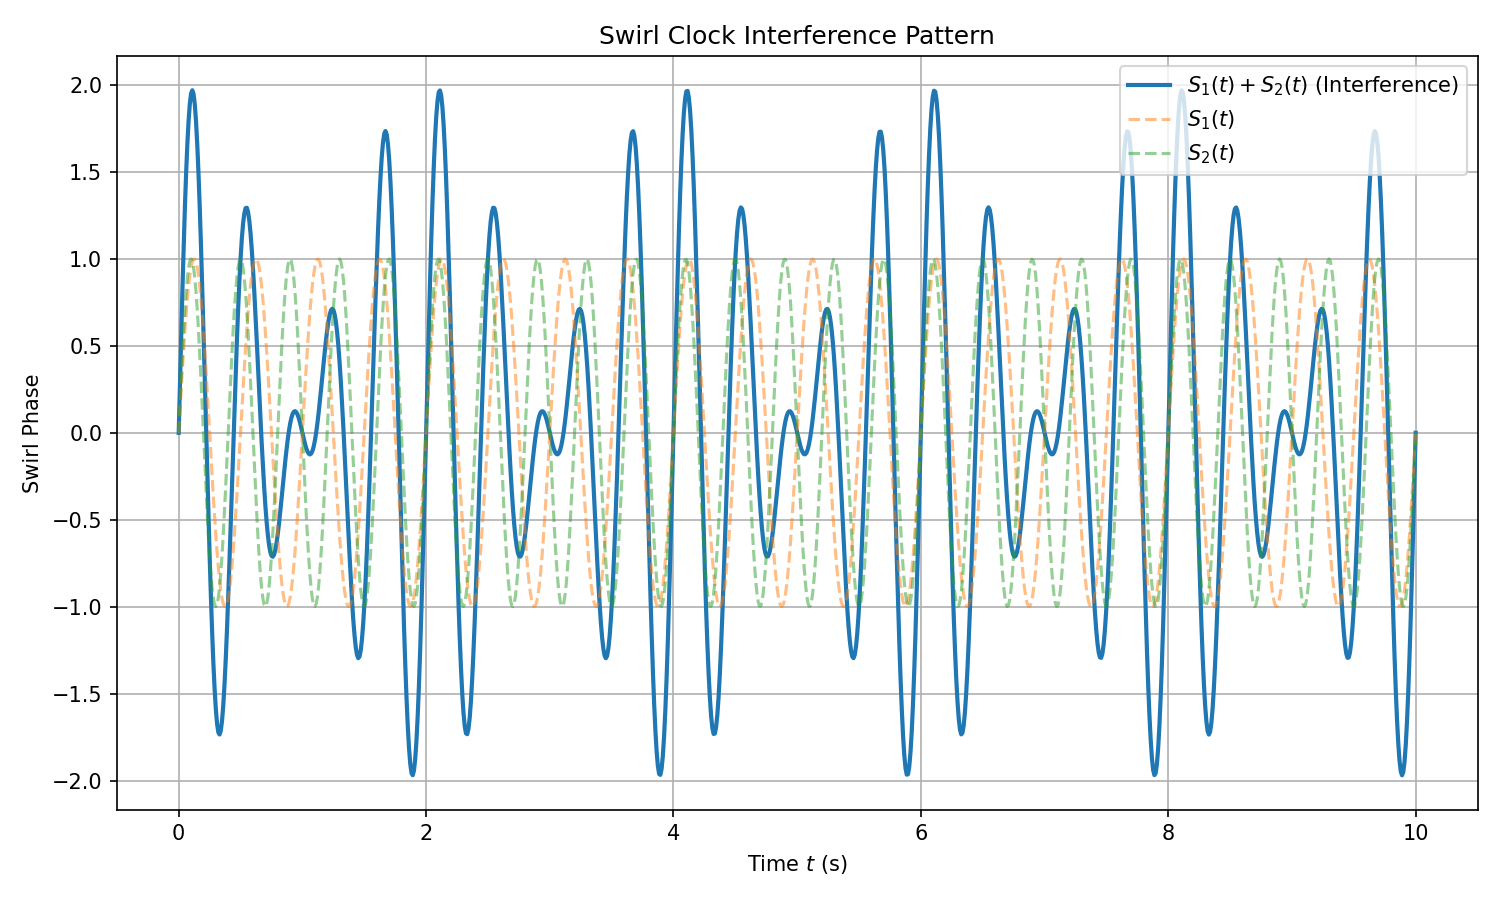
\includegraphics[width=0.8\textwidth]{../images/SwirlClockInterference}
    \caption{Interference between two swirl clocks with angular frequencies $\omega_1 = 4\pi$ and $\omega_2 = 5\pi$. The phase difference leads to beat structures and modulation patterns—analogous to quantum spinor dynamics and timing gates in ætheric systems.}
    \label{fig:swirl_interference}
\end{figure}

\subsection*{2. Energy Growth from Kairos Moment}
\begin{figure}[H]
    \centering
    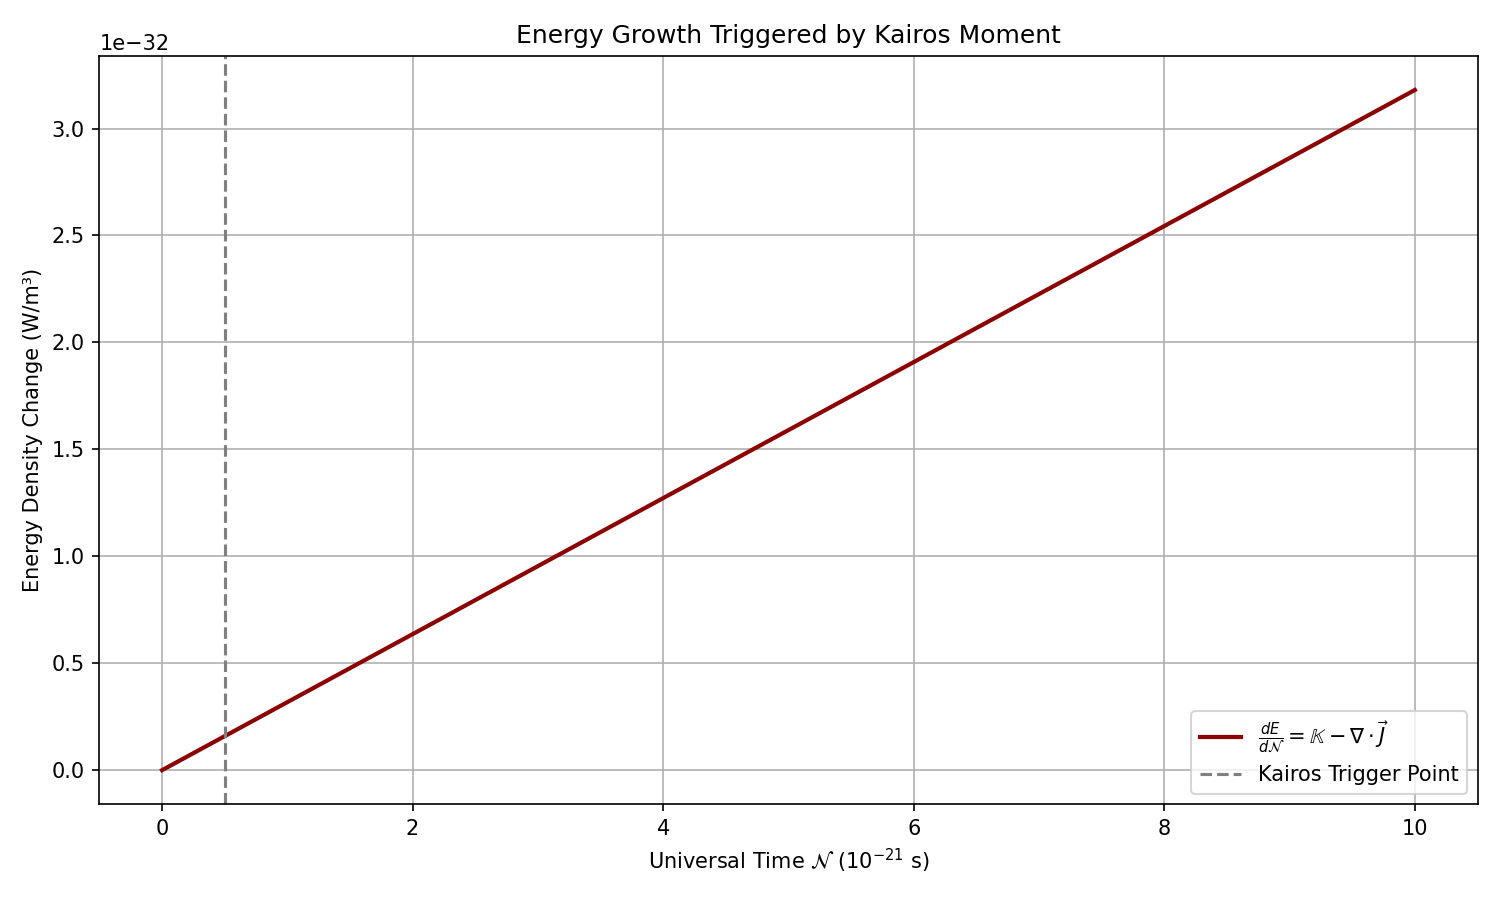
\includegraphics[width=0.8\textwidth]{../images/SwirlClockInterference2}
    \caption{Temporal evolution of energy density in æther, showing energy injection at a Kairos moment ($\mathbb{K}$) minus the divergence of energy flux $\nabla \cdot \vec{J}$. The slope reflects the conservation law $\dv{E}{\mathcal{N}} + \nabla \cdot \vec{J} = \mathbb{K}$.}
    \label{fig:kairos_energy}
\end{figure}

\subsection*{3. Swirl-Modulated Field Tensor}
\begin{figure}[H]
    \centering
    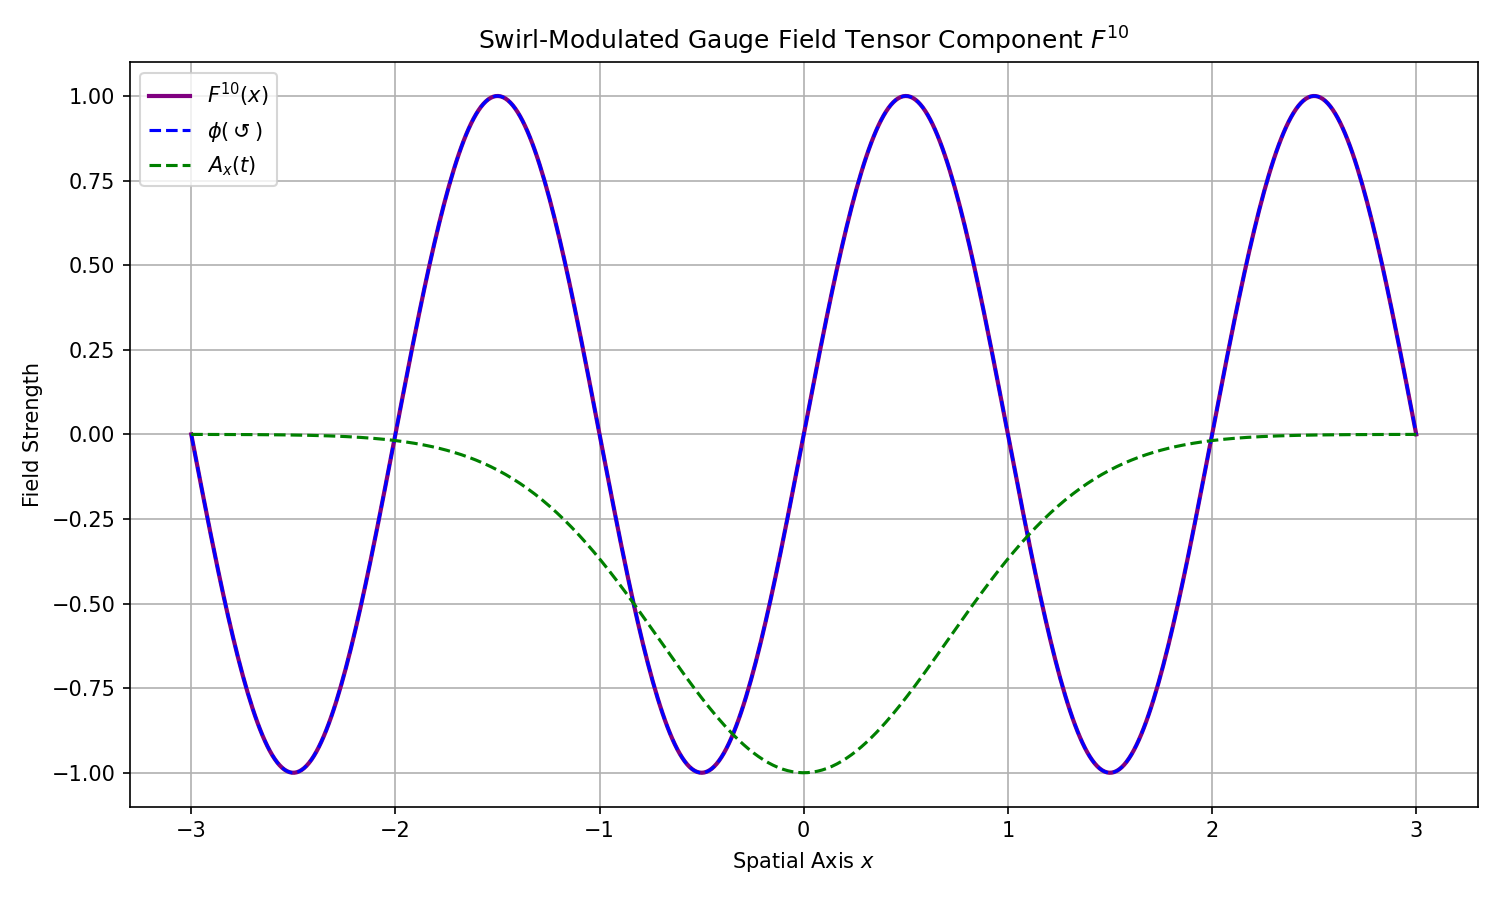
\includegraphics[width=0.8\textwidth]{../images/SwirlClockInterference3}
    \caption{Spatial variation of the gauge field tensor component $F^{1 0}$ under the influence of a swirl-phase-modulated potential $\phi(\circlearrowleft) = \lambda \sin(\theta(x))$ and a vector potential $A_x(t) = e^{-x^2} \cos(\omega t)$. This illustrates how topological internal structures alter observable field properties.}
    \label{fig:swirl_tensor}
\end{figure}


\end{document}